\documentclass[conference]{IEEEtran}
\IEEEoverridecommandlockouts
% The preceding line is only needed to identify funding in the first footnote. If that is unneeded, please comment it out.
\usepackage[noadjust]{cite}
\usepackage{filecontents}
\usepackage{amsmath,amssymb,amsfonts}
\usepackage{algorithmic}
\usepackage{graphicx}
\usepackage{textcomp}
\def\BibTeX{{\rm B\kern-.05em{\sc i\kern-.025em b}\kern-.08em
    T\kern-.1667em\lower.7ex\hbox{E}\kern-.125emX}}
\begin{document}

\title{Morphometry landmarks detection by convolutional neural network}

\author{\IEEEauthorblockN{Van Linh LE}
\IEEEauthorblockA{\textit{LaBRI - CNRS 5800, France} \\
\textit{ITDLU - Dalat University, Vietnam}\\
van-linh.le@labri.fr/ \\
linhlv@dlu.edu.vn}
\and
\IEEEauthorblockN{Marie BEURTON-AIMAR}
\IEEEauthorblockA{\textit{LaBRI - CNRS 5800} \\
\textit{Bordeaux University}\\
Talence, France \\
beurton@labri.fr}
\and
\IEEEauthorblockN{Akka ZEMMARI}
\IEEEauthorblockA{\textit{LaBRI - CNRS 5800} \\
\textit{Bordeaux University}\\
Talence, France \\
zemmari@labri.fr}
\and
\IEEEauthorblockN{Nicolas PARISEY}
\IEEEauthorblockA{\textit{IGEPP} \\
\textit{INRA 1349}\\
Le Rheu, France \\
nparisey@rennes.inra.fr}

}

\maketitle

\begin{abstract}
Morphometric analysis is general method applied on organisms and are useful to appraise the covariances between the ecological factors and the organisms(shape, size, form,...). In which, landmark-based morphometric is known as one of the approaches to analyze the characteristics of organisms. Finding enough the landmarks can give to the biologist a comprehensive description of organism shape. In this study, we propose a convolutional neural network (CNN) to predict the landmarks on biological images. The network is designed as a pipeline of the layers, it was trained with a set of manually landmarks examples. Then, the network is used to provide the morphometric landmarks on biological images automatically. The coordinates of predicted landmarks are evaluated by calculating the correlation coefficient with the manual coordinates which given by the biologists. Besides, the evaluations of the distances between predicted and manual landmarks are also given. The network is implemented by Python on Lassagne framework.
\end{abstract}

\begin{IEEEkeywords}
Morphometry, biological, landmarks, CNN
\end{IEEEkeywords}

\section{Introduction}
Morphometry analysis refers to measure the topography of an object, a notion that includes the shape and size\cite{•}. Morphometry analysis is generally applied to organisms. In biology, the biologist can work with several pieces of information from organisms such as lengths, widths, masses, angles,... to analyze the interaction of environment to the developmental of organisms. Besides the traditional information, the landmark is known as one of the characteristics to analyze the shape. Instead of collecting all information, the shape is determined by a finite set of points, called landmarks. The landmarks are the points that store the important information about the shape of the object, for example, four corners of the rectangle are four landmarks of a rectangle. Normally, the landmarks are along on the outline of the object but in some special cases, it has been defined inside the object. Morphometry landmarks are a kind of points-of-interest, they are directly linked to the animal anatomy. In our study, the morphometric landmarks are specific points defined by the biologists. They are used in many biological studies and include the classification tasks. Manual landmarks identification is time-consuming and difficult to re-procedure.

This work introduces a method for automatic detection the landmarks on biological images. The main idea consists design and trains a convolutional neural network\cite{•} with a set of manual landmarks. By this way, the trained network will be able to detect the morphometry landmarks on biological images. The dataset that used to study including 293 beetles images from Brittany lands. All the images are presented in RGB color with two dimensional. For each beetle, the biologists took images of five parts: left and right mandibles, head, body, and pronotum. For every image, a set of landmarks has been manually determined by experts. In the last our work, a method has been presented to determine the landmarks on left and right mandibles. This method is based on the image processing techniques \cite{•}. In the context of this work, we work on the dataset of pronotum images (Fig.\ref{figpronotum}). For each pronotum image, a set of 8 manual landmarks have been set by the biologists. The coordinates of manual landmarks as the input to train the network. During the first phase, a number of 260 images and their manual landmarks are used to train and validate the network. The remaining images are used to evaluate the output model of the network in the second phase.
\begin{figure}[htbp]
	\centerline{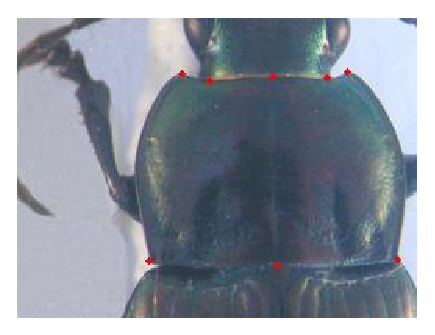
\includegraphics[scale=0.8]{images/pronotum}}
	\caption{An example of pronotum with manual landmarks}
	\label{figpronotum}
\end{figure}

In the next section, we study several related works to determine the landmarks on 2D images by CNN. Section 3 presents the network, its parameters, and the implementation. All the experiments and analysing the results will be detailed in section 4.
\section{Related works}
In recent years, deep learning is known as a solution for computer vision literature. Using convolutional network to learn the vision features or to detect the important features on the images have achieved better results in many domains such as image classification \cite{•}, face detection and pose estimation\cite{•}, handwritten detection\cite{•} and key points (landmarks) identification \cite{•}. The landmarks are not only used in biology, they appear in many domains with many applications. 

In the field of facial keypoint detection, Yi Sun et al.\cite{•} proposed cascaded convolutional networks to predict five facial points (points stay on the human face): \textit{left eye center, right eye center, nose, left mouth corner, and right mouth corner}. They cascade three levels of the convolutional network to predict the facial points: In the first level, the networks are designed to predict several landmarks together by covering the whole face; the networks in the second and the third level are used to predict each landmark on the face. They take the patches centered at the predicted positions of previous levels as input and try to improve the accuracy of predicted positions. Zhanpeng Zhang et al\cite{•} proposed a \textit{Tasks-Constrained Deep Convolutional Network} to optimize facial landmarks detection. The model determined the facial landmarks with a set of related tasks such as head pose estimation, gender classification, age estimation, face recognition, or facial attribute inference. Firstly, all the images are used as the input, their output spaces the images into several tasks. Then, the network is applied to determine the landmarks on the images of each task. 

In biology field, Cintas et al\cite{•} has introduced a network to predict the landmarks on human ears. The network was designed to receive the images with the size of $96 \times 96$ as the inputs. After training, the network has the ability to predict 45 landmarks and semi-landmarks on human ears. In the proposed architecture, the network with three times repeated of a structure includes two convolutional layers with the filters, followed by maximum pooling and dropout layers. The structures then adding two full-connected layers and a dropout layer. At the end, an output layer with 90 output units corresponding with 45 landmarks is hired to provide the position of the predicted landmarks.

\section{Method and implementation}
\subsection{Convolutional neural networks}
\subsection{Data and preprocessing data}
The images come from a collection of 293 beetles from Brittany lands. All the images are taken with the same camera under same conditions with a $3264 \times 2448$ resolutions. For each specific part, a set of manual landmarks has been determined by biologists, \textit{for examples, 8 landmarks for pronotum, 16 landmarks for the left mandible, 18 landmarks for right mandible}. In the content of this study, we work on pronotum part of beetle. The provided dataset contains 293 images, each image with 8 landmarks provided by biologists. The dataset was split into a training set with 260 images (training and validation) and a testing set of 33 images. During the training, the network learned the information through a pair of \textit{(image, landmarks)} in training set. At the testing phase, the image without landmarks was given to the trained network and the predicted landmarks will be given at the output.

Because the resolution of the image is large, it becomes a difficulty for the network. During training and testing, the images are down-sampling to the new resolution of $256 \times 192$. Besides, the landmark coordinates of the image are also scaled to suit their new resolution.
\subsection{Network architecture and training}
The CNN was designed and trained for performing an automatic landmarks detection on pronotum images. The network consists several common layers in the neural network with different learnable parameters. It takes a single channel pronotum image with the size of  $256 \times 192$ as the input. Before entering the network, the brightness of pixels in the image are scaled to $[0,1]$, instead of $[0,255]$. Fig.\ref{figarch} shows the architecture of proposed network. The structure consists of a convolution layer with square filter, followed with a \textit{maximum} pooling and dropout layer. This structure is repeated three times in the architecture with the differences of filter size, number of features and probability values. The difference of layer parameters provides to the network the ability to study the features at different levels. In this structure, all \textit{max} pooling layers have the same size $2 \times 2$ for the filters. While, the number of filters and the size of filters at convolution layers are different. The number of filters is increased from the first convolution layer to the third convolution layer. The values of the filters are 32, 64, and 128, respectively. Besides, the size of filters are also not the same: $3 \times 3$, $2 \times 2$, and $2 \times 2$. The probability values used for dropout layers are $0.1$, $0.2$, and $0.3$.

\begin{figure}[htbp]
	\centerline{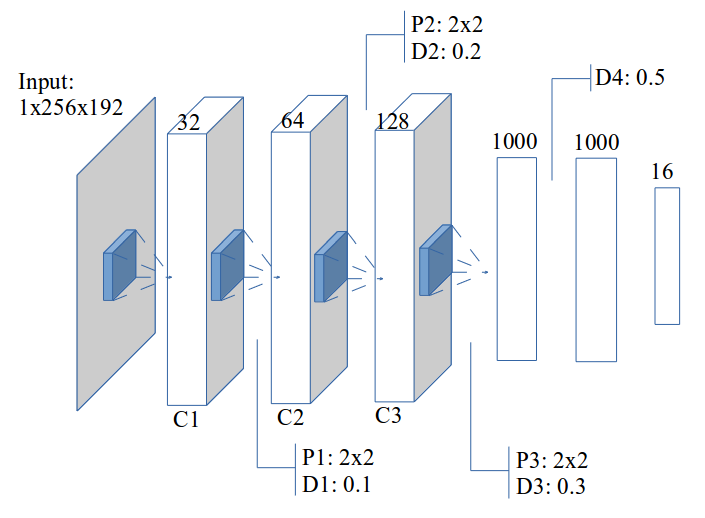
\includegraphics[scale=0.3]{images/architecture}}
	\caption{The architecture of proposed network}
	\label{figarch}
\end{figure}

After three feature extraction structures, the architecture contains two full connected layers with 1000 units per each layer and a dropout layer between them. The probability value of this layer is set to $0.5$. The output layer contains 16 units corresponding to the coordinates of eight predicted landmarks. The implementation of this architecture used Python on Lassagne framework\cite{lasagne} which allows to train the network on GPU. The training process took around 3 hours using NVIDIA TITAN X cards.
\subsection{Overfitting problem}
The proposed network has a large number of learnable parameters. In addition, the size of the dataset is limited, this means that overfitting will occur during the training process. Because the network works on  gray-scale image and mostly the processes compute the value from the pixels. So, we have applied two rules to enlarge the size of the dataset.

The first rule was applied to change the value of each channel in the original image. According to this rule, a constant is adding to a channel of RGB image and for each time, we just change the value of one of three channels. For example, from an original RGB image, if we add a constant $c = 10$ to the red channel, we will obtain a new image with the values at red channel are greater than the red channel of original image a value of 10. By this way, we can generate three new RGB images from a RGB image.

The second rule is splitting the channels of RGB images. It means that we separate the channels of RGB into three gray-scale images. This work seems like right because the network works on single-channel images. At the end, we can generate six version from an image, the total number of images that used to train and validate is $260 \times 7 = 1820$ images (six versions and original image). The number of images that used for training and validation is split randomly by a ratio that has been set during setup the network.
\section{Results}
The dataset has been built by the biologists. It includes the images and manual landmarks. So, we can use the manual landmarks coordinates as ground truth to evaluate the coordinates of predicted landmarks. In the context of deep learning, landmark prediction can see as the regression problem. Therefore, the quality metric is used to evaluate the results. In particular, we use root mean square error (RMSE) to compute the accuracy of the implemented architecture. To have the predicted coordinates of all landmarks in all the images, the network was trained many times with different training dataset and was tested on the corresponding test set.

\begin{figure}[htbp]
	\centerline{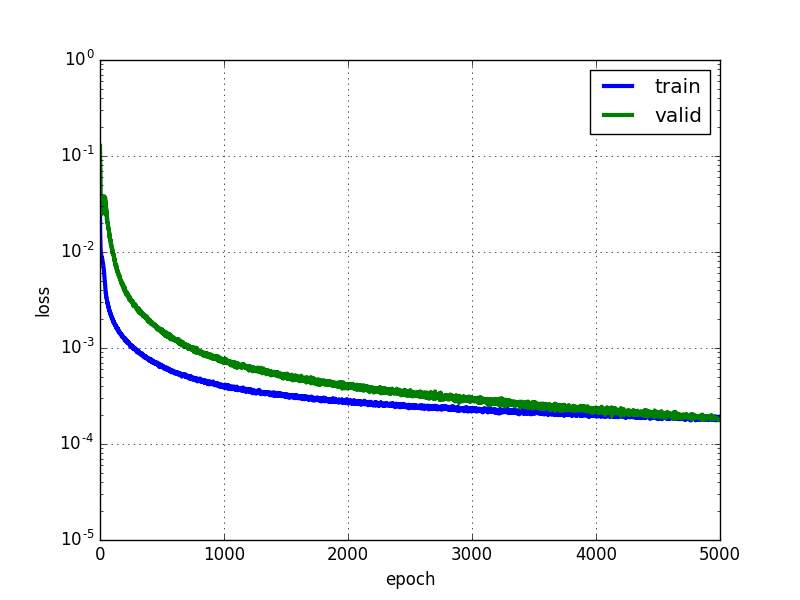
\includegraphics[scale=0.35]{images/loss_v16}}
	\caption{Learning curves of the network. The blue curve presents RMSE on training set, the green curve presents the validation error}
	\label{figloss}
\end{figure}

The learning curves in Fig.\ref{figloss} show the training error and the validation error of one training (and validation) time of the network. Fig.\ref{figrsexample} shows the predicted landmarks on an unseen image in the test set.

\begin{figure}[htbp]
	\centerline{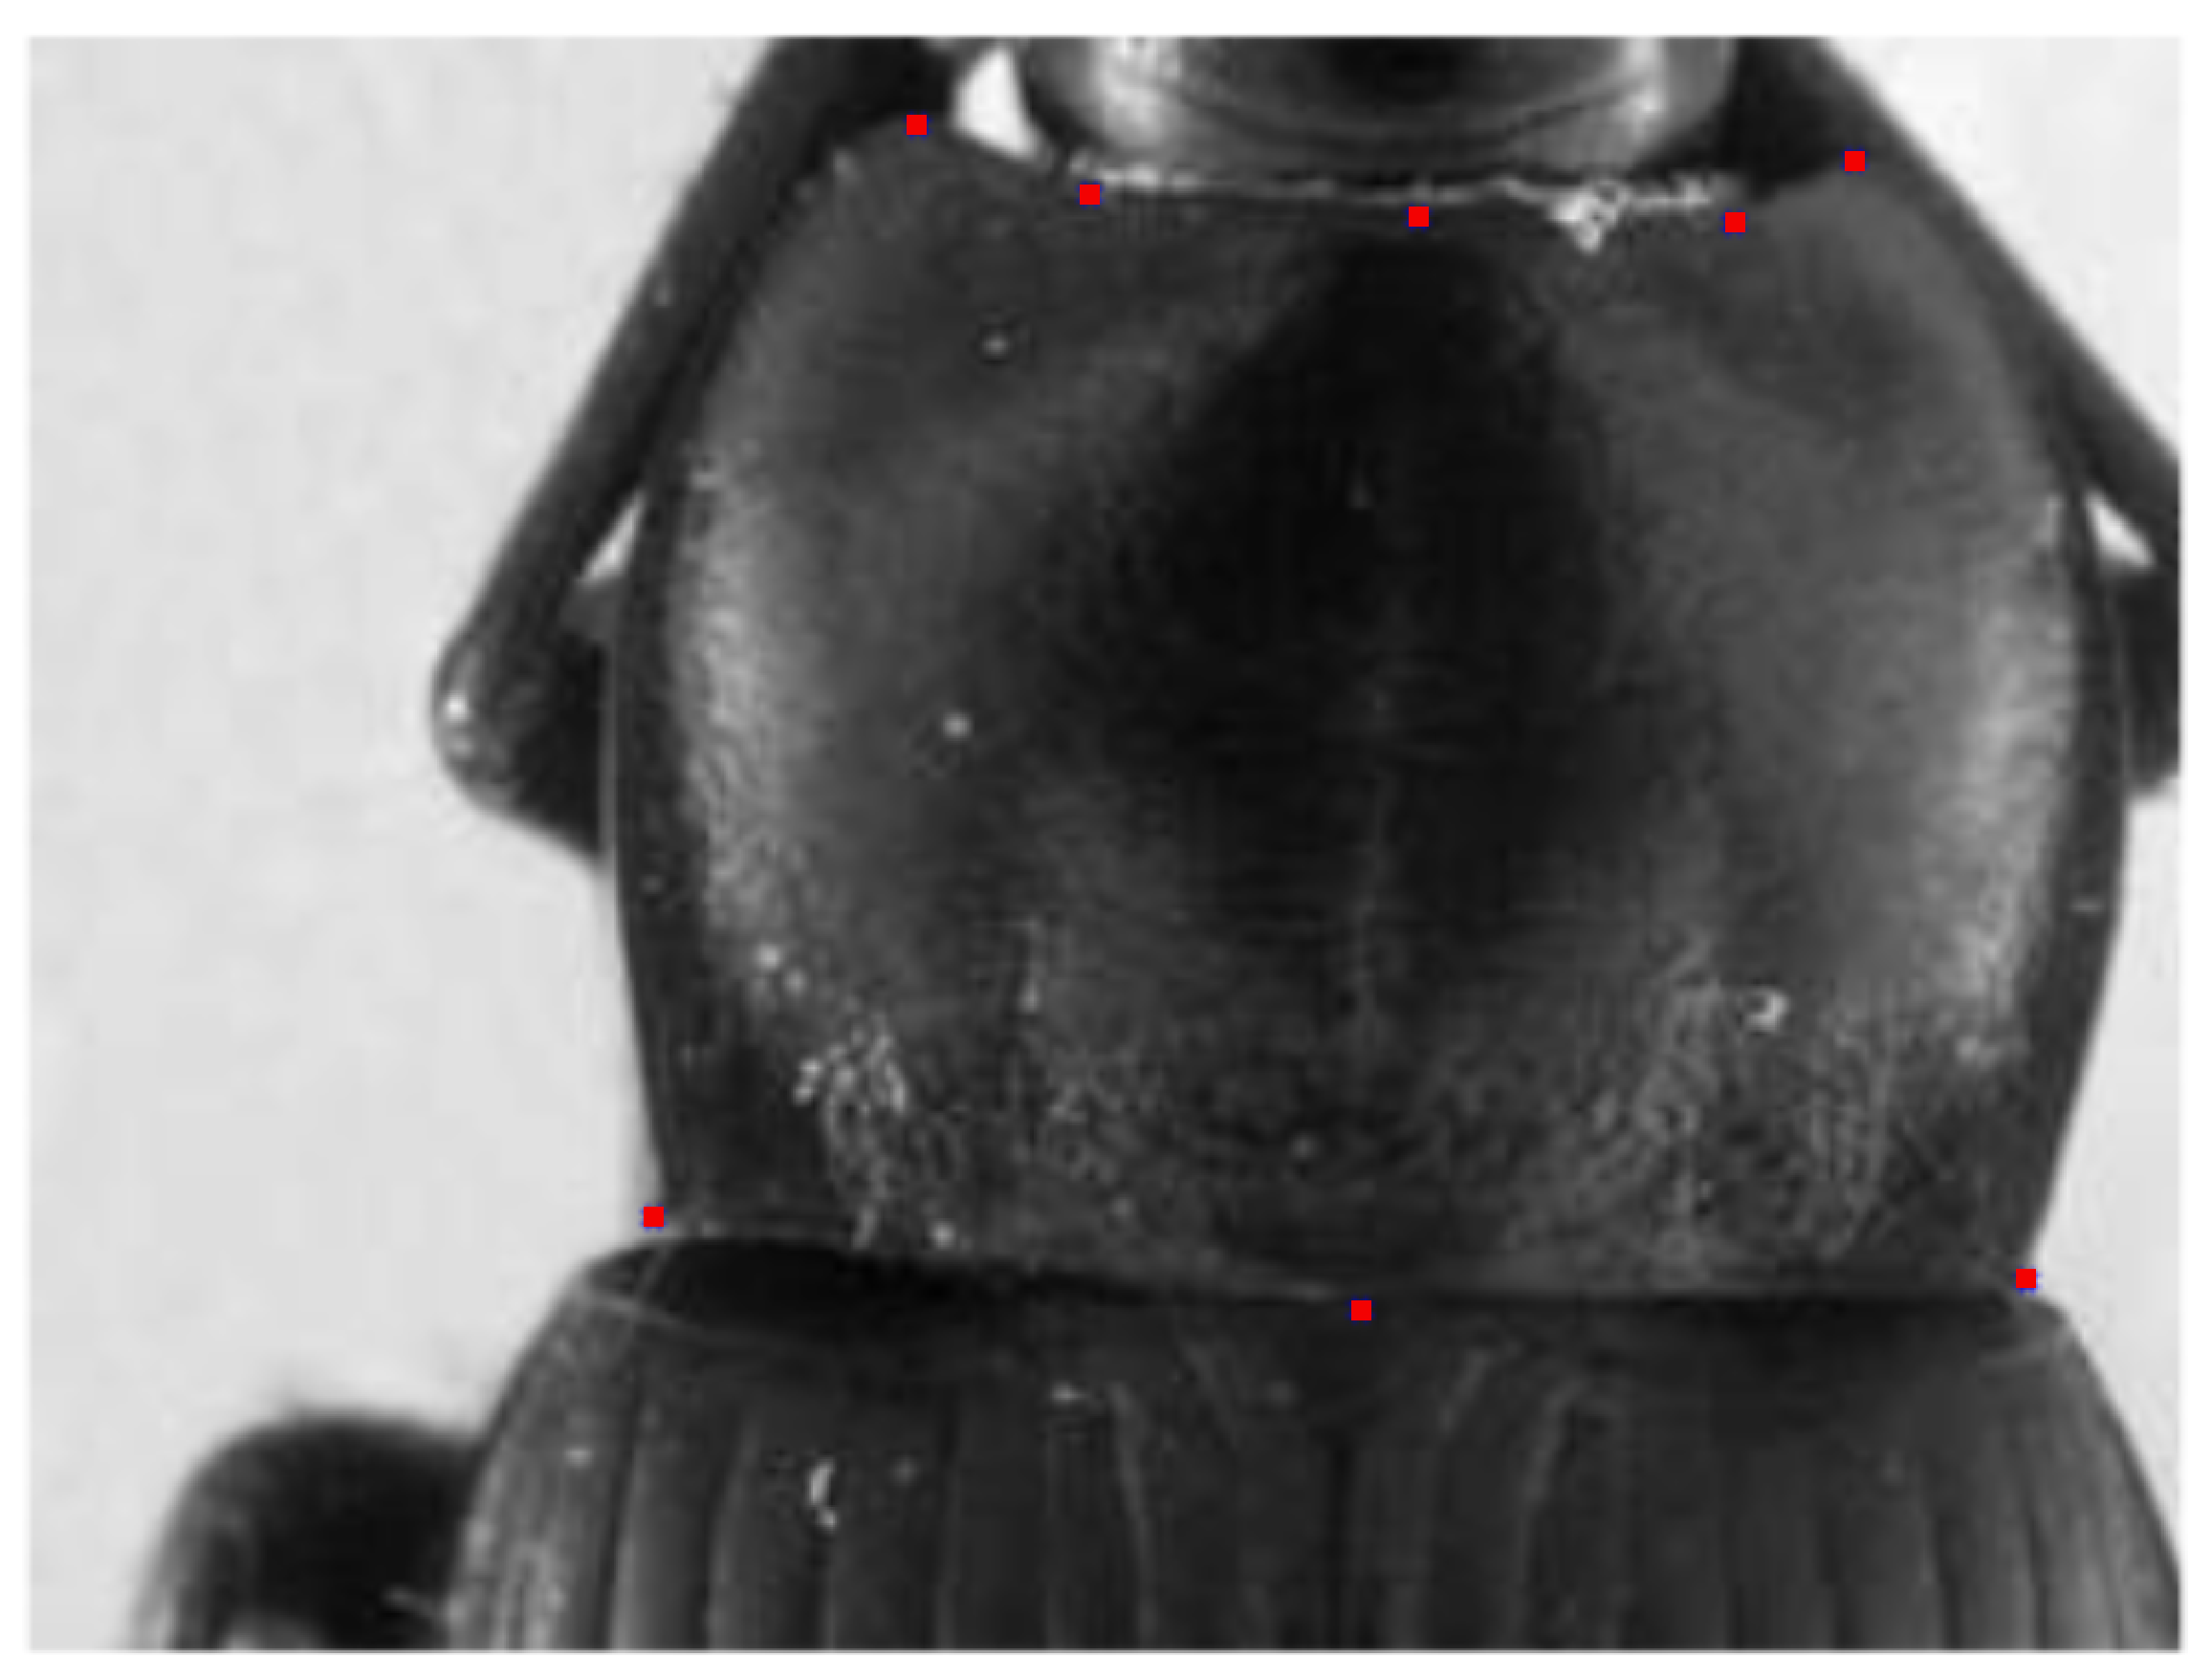
\includegraphics[scale=0.18]{images/plandmark}}
	\caption{The predicted landmarks on an image in test set (red points)}
	\label{figrsexample}
\end{figure}
For a comprehensive evaluation of the efficacy of the network. The correlation coefficient on the coordinates of predicted landmarks is calculated by using three methods: Pearson\cite{•}, Spearman\cite{•}, and Kendall\cite{•}. These results are shown in Table.\ref{tab1}.
\begin{table}[htbp]
\caption{The correlation coefficient of predicted landmarks on several correlation methods}
\begin{center}
\begin{tabular}{|c|c|c|}
\hline
\textbf{Method} & \textbf{x-correlation} & \textbf{y-correlation} \\ \hline
Pearson & 0.9970585 & 0.9978605 \\ \hline
Spearman & 0.9942475 & 0.9859642 \\ \hline
Kendall & 0.9430501 & 0.9067739 \\ \hline
\end{tabular}
\label{tab1}
\end{center}
\end{table}

Besides the coefficient, the distance from predicted landmarks to manual landmarks deserves attention also. Firstly, the distance between them is calculated. Then, the standard deviation is used to quantify the dispersion of a set of distance. Table.\ref{tab2} shows the average error distance given on each landmark. Fig.\ref{figchart} shows the proportion of acceptable landmarks. In our case, a predicted landmark is acceptable if the distance between it and corresponding manual landmarks is less than the average distance plus a value of standard deviation. Most of the landmarks have been detected with the accuracy greater than $70\%$. However, we can see a vast difference between the correlation coefficient results and the proportions on each landmark.

\begin{table}[htbp]
\caption{The average distance on each landmark}
\begin{center}
\begin{tabular}{|c|p{1.5cm}|}
\hline
\textbf{$\#$Landmark} & \textbf{Distance} \\ \hline
1 & 4.002  \\ \hline
2 & 4.4831 \\ \hline
3 & 4.2959 \\ \hline
4 & 4.3865 \\ \hline
5 & 4.2925 \\ \hline
6 & 5.3631 \\ \hline
7 & 4.636 \\ \hline
8 & 4.9363 \\ \hline
\end{tabular}
\label{tab2}
\end{center}
\end{table}

\begin{figure}[htbp]
	\centerline{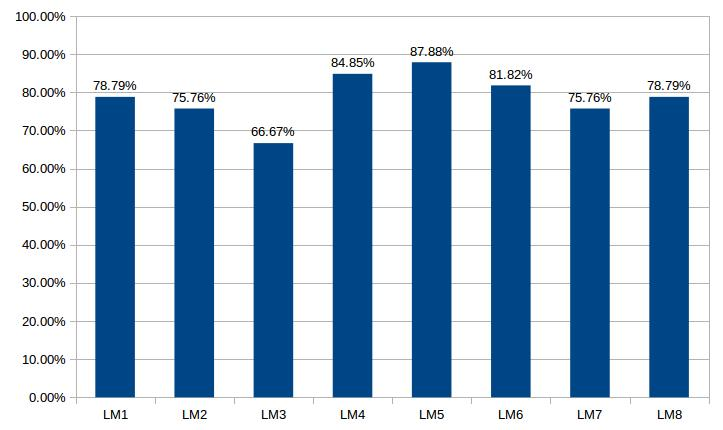
\includegraphics[scale=0.35]{images/pronotum_pmodel_statistic}}
	\caption{The proportion of acceptable predicted landmarks}
	\label{figchart}
\end{figure}
\section{Conclusion and future works}
We present a method for landmarks prediction on beetle images. The method used the convolutional neural network for automatic detection landmarks. After training with the manual landmarks which given by the biologist, the network is possible to predict the landmarks on unseen images. The model is implemented using open source tools. The results from the testing period are evaluated by several different methods. Some of them has been given the good coefficient. The quality of prediction can be used to replace for manual landmarks in some aspect.

Finally, using the convolutional network to predict the landmarks on biological images promising the good results. However, when we expect more about the accuracy of predicted landmarks, the result of this work is not enough. Therefore, future research in landmarking identification appears as a improve the worth exploring.

\section*{References}

Please number citations consecutively within brackets \cite{b1}. The 
sentence punctuation follows the bracket \cite{b2}. Refer simply to the reference 
number, as in \cite{b3}---do not use ``Ref. \cite{b3}'' or ``reference \cite{b3}'' except at 
the beginning of a sentence: ``Reference \cite{b3} was the first $\ldots$''

Number footnotes separately in superscripts. Place the actual footnote at 
the bottom of the column in which it was cited. Do not put footnotes in the 
abstract or reference list. Use letters for table footnotes.

Unless there are six authors or more give all authors' names; do not use 
``et al.''. Papers that have not been published, even if they have been 
submitted for publication, should be cited as ``unpublished'' \cite{b4}. Papers 
that have been accepted for publication should be cited as ``in press'' \cite{b5}. 
Capitalize only the first word in a paper title, except for proper nouns and 
element symbols.

For papers published in translation journals, please give the English 
citation first, followed by the original foreign-language citation \cite{b6}.

%\begin{thebibliography}{00}
%\bibitem{b1} G. Eason, B. Noble, and I. N. Sneddon, ``On certain integrals of Lipschitz-Hankel type involving products of Bessel functions,'' Phil. Trans. Roy. Soc. London, vol. A247, pp. 529--551, April 1955.
%\bibitem{b2} J. Clerk Maxwell, A Treatise on Electricity and Magnetism, 3rd ed., vol. 2. Oxford: Clarendon, 1892, pp.68--73.
%\bibitem{b3} I. S. Jacobs and C. P. Bean, ``Fine particles, thin films and exchange anisotropy,'' in Magnetism, vol. III, G. T. Rado and H. Suhl, Eds. New York: Academic, 1963, pp. 271--350.
%\bibitem{b4} K. Elissa, ``Title of paper if known,'' unpublished.
%\bibitem{b5} R. Nicole, ``Title of paper with only first word capitalized,'' J. Name Stand. Abbrev., in press.
%\bibitem{b6} Y. Yorozu, M. Hirano, K. Oka, and Y. Tagawa, ``Electron spectroscopy studies on magneto-optical media and plastic substrate interface,'' IEEE Transl. J. Magn. Japan, vol. 2, pp. 740--741, August 1987 [Digests 9th Annual Conf. Magnetics Japan, p. 301, 1982].
%\bibitem{b7} M. Young, The Technical Writer's Handbook. Mill Valley, CA: University Science, 1989.

%\end{thebibliography}
\bibliographystyle{IEEEtran}
\bibliography{includes/references}
\end{document}
